\documentclass[twoside]{book}

% Packages required by doxygen
\usepackage{fixltx2e}
\usepackage{calc}
\usepackage{doxygen}
\usepackage[export]{adjustbox} % also loads graphicx
\usepackage{graphicx}
\usepackage[utf8]{inputenc}
\usepackage{makeidx}
\usepackage{multicol}
\usepackage{multirow}
\PassOptionsToPackage{warn}{textcomp}
\usepackage{textcomp}
\usepackage[nointegrals]{wasysym}
\usepackage[table]{xcolor}

% Font selection
\usepackage[T1]{fontenc}
\usepackage[scaled=.90]{helvet}
\usepackage{courier}
\usepackage{amssymb}
\usepackage{sectsty}
\renewcommand{\familydefault}{\sfdefault}
\allsectionsfont{%
  \fontseries{bc}\selectfont%
  \color{darkgray}%
}
\renewcommand{\DoxyLabelFont}{%
  \fontseries{bc}\selectfont%
  \color{darkgray}%
}
\newcommand{\+}{\discretionary{\mbox{\scriptsize$\hookleftarrow$}}{}{}}

% Page & text layout
\usepackage{geometry}
\geometry{%
  a4paper,%
  top=2.5cm,%
  bottom=2.5cm,%
  left=2.5cm,%
  right=2.5cm%
}
\tolerance=750
\hfuzz=15pt
\hbadness=750
\setlength{\emergencystretch}{15pt}
\setlength{\parindent}{0cm}
\setlength{\parskip}{3ex plus 2ex minus 2ex}
\makeatletter
\renewcommand{\paragraph}{%
  \@startsection{paragraph}{4}{0ex}{-1.0ex}{1.0ex}{%
    \normalfont\normalsize\bfseries\SS@parafont%
  }%
}
\renewcommand{\subparagraph}{%
  \@startsection{subparagraph}{5}{0ex}{-1.0ex}{1.0ex}{%
    \normalfont\normalsize\bfseries\SS@subparafont%
  }%
}
\makeatother

% Headers & footers
\usepackage{fancyhdr}
\pagestyle{fancyplain}
\fancyhead[LE]{\fancyplain{}{\bfseries\thepage}}
\fancyhead[CE]{\fancyplain{}{}}
\fancyhead[RE]{\fancyplain{}{\bfseries\leftmark}}
\fancyhead[LO]{\fancyplain{}{\bfseries\rightmark}}
\fancyhead[CO]{\fancyplain{}{}}
\fancyhead[RO]{\fancyplain{}{\bfseries\thepage}}
\fancyfoot[LE]{\fancyplain{}{}}
\fancyfoot[CE]{\fancyplain{}{}}
\fancyfoot[RE]{\fancyplain{}{\bfseries\scriptsize Generated by Doxygen }}
\fancyfoot[LO]{\fancyplain{}{\bfseries\scriptsize Generated by Doxygen }}
\fancyfoot[CO]{\fancyplain{}{}}
\fancyfoot[RO]{\fancyplain{}{}}
\renewcommand{\footrulewidth}{0.4pt}
\renewcommand{\chaptermark}[1]{%
  \markboth{#1}{}%
}
\renewcommand{\sectionmark}[1]{%
  \markright{\thesection\ #1}%
}

% Indices & bibliography
\usepackage{natbib}
\usepackage[titles]{tocloft}
\setcounter{tocdepth}{3}
\setcounter{secnumdepth}{5}
\makeindex

% Hyperlinks (required, but should be loaded last)
\usepackage{ifpdf}
\ifpdf
  \usepackage[pdftex,pagebackref=true]{hyperref}
\else
  \usepackage[ps2pdf,pagebackref=true]{hyperref}
\fi
\hypersetup{%
  colorlinks=true,%
  linkcolor=blue,%
  citecolor=blue,%
  unicode%
}

% Custom commands
\newcommand{\clearemptydoublepage}{%
  \newpage{\pagestyle{empty}\cleardoublepage}%
}

\usepackage{caption}
\captionsetup{labelsep=space,justification=centering,font={bf},singlelinecheck=off,skip=4pt,position=top}

%===== C O N T E N T S =====

\begin{document}

% Titlepage & ToC
\hypersetup{pageanchor=false,
             bookmarksnumbered=true,
             pdfencoding=unicode
            }
\pagenumbering{roman}
\begin{titlepage}
\vspace*{7cm}
\begin{center}%
{\Large Treasure Run project }\\
\vspace*{1cm}
{\large Generated by Doxygen 1.8.11}\\
\end{center}
\end{titlepage}
\clearemptydoublepage
\tableofcontents
\clearemptydoublepage
\pagenumbering{arabic}
\hypersetup{pageanchor=true}

%--- Begin generated contents ---
\chapter{Namespace Index}
\section{Namespace List}
Here is a list of all documented namespaces with brief descriptions\+:\begin{DoxyCompactList}
\item\contentsline{section}{\hyperlink{namespace_ui}{Ui} }{\pageref{namespace_ui}}{}
\end{DoxyCompactList}

\chapter{Hierarchical Index}
\section{Class Hierarchy}
This inheritance list is sorted roughly, but not completely, alphabetically\+:\begin{DoxyCompactList}
\item Q\+Graphics\+Pixmap\+Item\begin{DoxyCompactList}
\item \contentsline{section}{Enemy}{\pageref{class_enemy}}{}
\item \contentsline{section}{Player}{\pageref{class_player}}{}
\item \contentsline{section}{Weapon}{\pageref{class_weapon}}{}
\end{DoxyCompactList}
\item Q\+Graphics\+Text\+Item\begin{DoxyCompactList}
\item \contentsline{section}{Health}{\pageref{class_health}}{}
\item \contentsline{section}{Score}{\pageref{class_score}}{}
\item \contentsline{section}{Weaponscore}{\pageref{class_weaponscore}}{}
\end{DoxyCompactList}
\item Q\+Graphics\+View\begin{DoxyCompactList}
\item \contentsline{section}{Game}{\pageref{class_game}}{}
\end{DoxyCompactList}
\item Q\+Main\+Window\begin{DoxyCompactList}
\item \contentsline{section}{Main\+Window}{\pageref{class_main_window}}{}
\end{DoxyCompactList}
\item Q\+Object\begin{DoxyCompactList}
\item \contentsline{section}{Enemy}{\pageref{class_enemy}}{}
\item \contentsline{section}{Player}{\pageref{class_player}}{}
\item \contentsline{section}{Weapon}{\pageref{class_weapon}}{}
\end{DoxyCompactList}
\end{DoxyCompactList}

\chapter{Class Index}
\section{Class List}
Here are the classes, structs, unions and interfaces with brief descriptions\+:\begin{DoxyCompactList}
\item\contentsline{section}{\hyperlink{class_enemy}{Enemy} \\*$<$ To make the graphic item }{\pageref{class_enemy}}{}
\item\contentsline{section}{\hyperlink{class_game}{Game} }{\pageref{class_game}}{}
\item\contentsline{section}{\hyperlink{class_health}{Health} }{\pageref{class_health}}{}
\item\contentsline{section}{\hyperlink{class_main_window}{Main\+Window} }{\pageref{class_main_window}}{}
\item\contentsline{section}{\hyperlink{class_player}{Player} }{\pageref{class_player}}{}
\item\contentsline{section}{\hyperlink{class_score}{Score} }{\pageref{class_score}}{}
\item\contentsline{section}{\hyperlink{class_weapon}{Weapon} \\*$<$For implementing graphics }{\pageref{class_weapon}}{}
\item\contentsline{section}{\hyperlink{class_weaponscore}{Weaponscore} }{\pageref{class_weaponscore}}{}
\end{DoxyCompactList}

\chapter{Namespace Documentation}
\hypertarget{namespace_ui}{}\section{Ui Namespace Reference}
\label{namespace_ui}\index{Ui@{Ui}}


\subsection{Detailed Description}
Katherine Wang Assignment 5 Description\+: Main window 
\chapter{Class Documentation}
\hypertarget{class_enemy}{}\section{Enemy Class Reference}
\label{class_enemy}\index{Enemy@{Enemy}}


$<$ To make the graphic item  




{\ttfamily \#include $<$enemy.\+h$>$}

Inheritance diagram for Enemy\+:\begin{figure}[H]
\begin{center}
\leavevmode
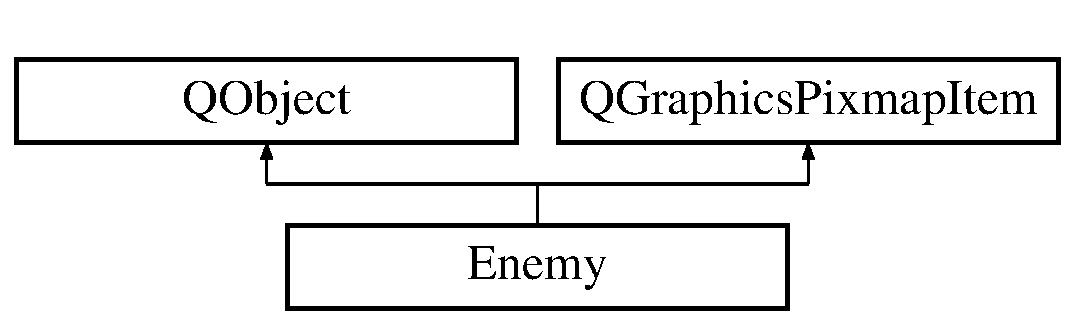
\includegraphics[height=2.000000cm]{class_enemy}
\end{center}
\end{figure}
\subsection*{Public Slots}
\begin{DoxyCompactItemize}
\item 
void \hyperlink{class_enemy_a9a398f8d12234f02563b27440aff7891}{move} ()
\begin{DoxyCompactList}\small\item\em $<$ slot marks a signal to a specific reaction \end{DoxyCompactList}\end{DoxyCompactItemize}
\subsection*{Public Member Functions}
\begin{DoxyCompactItemize}
\item 
\hyperlink{class_enemy_ac98fc516847e643f8e528f4bb7cbfa35}{Enemy} (Q\+Graphics\+Item $\ast$parent=0)
\begin{DoxyCompactList}\small\item\em $<$ signalling slots \end{DoxyCompactList}\end{DoxyCompactItemize}


\subsection{Detailed Description}
$<$ To make the graphic item 

$<$For implementing graphics $<$for signalling slots 

\subsection{Constructor \& Destructor Documentation}
\index{Enemy@{Enemy}!Enemy@{Enemy}}
\index{Enemy@{Enemy}!Enemy@{Enemy}}
\subsubsection[{\texorpdfstring{Enemy(\+Q\+Graphics\+Item $\ast$parent=0)}{Enemy(QGraphicsItem *parent=0)}}]{\setlength{\rightskip}{0pt plus 5cm}Enemy\+::\+Enemy (
\begin{DoxyParamCaption}
\item[{Q\+Graphics\+Item $\ast$}]{parent = {\ttfamily 0}}
\end{DoxyParamCaption}
)}\hypertarget{class_enemy_ac98fc516847e643f8e528f4bb7cbfa35}{}\label{class_enemy_ac98fc516847e643f8e528f4bb7cbfa35}


$<$ signalling slots 

\hyperlink{class_enemy_ac98fc516847e643f8e528f4bb7cbfa35}{Enemy\+::\+Enemy} constructor that creates the enemy and rotates the picture. It also connects the enemy to the UI.

enemy constructor $<$ Set a random position for the enemy

Draw the enemy size (rectangle)

connect and make a timer that makes the enemy move

$<$ object whose signal you want to connect, constructor, move.

$<$ setting timer\textquotesingle{}s time to 50 milliseconds. 

\subsection{Member Function Documentation}
\index{Enemy@{Enemy}!move@{move}}
\index{move@{move}!Enemy@{Enemy}}
\subsubsection[{\texorpdfstring{move}{move}}]{\setlength{\rightskip}{0pt plus 5cm}void Enemy\+::move (
\begin{DoxyParamCaption}
{}
\end{DoxyParamCaption}
)\hspace{0.3cm}{\ttfamily [slot]}}\hypertarget{class_enemy_a9a398f8d12234f02563b27440aff7891}{}\label{class_enemy_a9a398f8d12234f02563b27440aff7891}


$<$ slot marks a signal to a specific reaction 

\hyperlink{class_enemy_a9a398f8d12234f02563b27440aff7891}{Enemy\+::move} Moves the enemy vertically downwards. Will delete when the enemy is off the screen. Also causes the player to disappear if the player collides with a monster.

will make the enemy move if enemy collides with player, destroy both.

playing monster growl

decrease the health

when the health is = 0

remove both

moving enemy down

$<$ x() = current x, y() = current y

moving enemy down faster

$<$ x() = current x, y() = current y

moving enemy down even faster

$<$ x() = current x, y() = current y

delete the enemy when it\textquotesingle{}s off the screen 

The documentation for this class was generated from the following files\+:\begin{DoxyCompactItemize}
\item 
/\+Users/\+Katherine/\+Desktop/\+P\+I\+C 10\+C -\/ Winter 2015/\+Treasure Run Submission -\/ Hw8/enemy.\+h\item 
/\+Users/\+Katherine/\+Desktop/\+P\+I\+C 10\+C -\/ Winter 2015/\+Treasure Run Submission -\/ Hw8/enemy.\+cpp\end{DoxyCompactItemize}

\hypertarget{class_game}{}\section{Game Class Reference}
\label{class_game}\index{Game@{Game}}


{\ttfamily \#include $<$game.\+h$>$}

Inheritance diagram for Game\+:\begin{figure}[H]
\begin{center}
\leavevmode
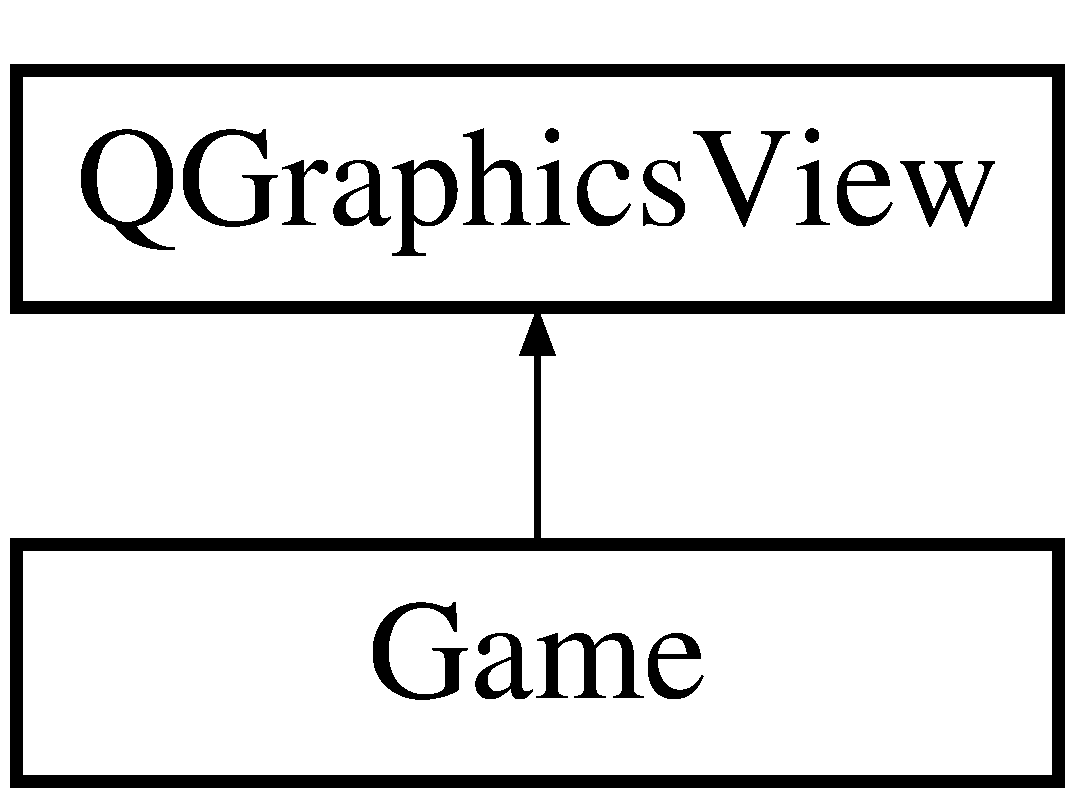
\includegraphics[height=2.000000cm]{class_game}
\end{center}
\end{figure}
\subsection*{Public Member Functions}
\begin{DoxyCompactItemize}
\item 
\hyperlink{class_game_ae3c64a8dd73de0a99849db8ec0e9a86c}{Game} (Q\+Widget $\ast$parent=0)
\end{DoxyCompactItemize}
\subsection*{Public Attributes}
\begin{DoxyCompactItemize}
\item 
\hyperlink{class_player}{Player} $\ast$ \hyperlink{class_game_abec70aa1c0269a9a7e171af4d79e08bf}{player}\hypertarget{class_game_abec70aa1c0269a9a7e171af4d79e08bf}{}\label{class_game_abec70aa1c0269a9a7e171af4d79e08bf}

\begin{DoxyCompactList}\small\item\em Creating player object. \end{DoxyCompactList}\item 
\hyperlink{class_score}{Score} $\ast$ \hyperlink{class_game_ad195acc6b5ee17a5a07fea0b7b4ff5e2}{score}\hypertarget{class_game_ad195acc6b5ee17a5a07fea0b7b4ff5e2}{}\label{class_game_ad195acc6b5ee17a5a07fea0b7b4ff5e2}

\begin{DoxyCompactList}\small\item\em Creating score object. \end{DoxyCompactList}\item 
\hyperlink{class_health}{Health} $\ast$ \hyperlink{class_game_a4cfa8ef83412c73d759b3965804f42aa}{health}\hypertarget{class_game_a4cfa8ef83412c73d759b3965804f42aa}{}\label{class_game_a4cfa8ef83412c73d759b3965804f42aa}

\begin{DoxyCompactList}\small\item\em Creating health object. \end{DoxyCompactList}\item 
\hyperlink{class_enemy}{Enemy} $\ast$ \hyperlink{class_game_aaaef99ac0f9bb6fc836e8195b0ea8756}{enemy}\hypertarget{class_game_aaaef99ac0f9bb6fc836e8195b0ea8756}{}\label{class_game_aaaef99ac0f9bb6fc836e8195b0ea8756}

\begin{DoxyCompactList}\small\item\em Creating enemy object. \end{DoxyCompactList}\item 
Q\+Graphics\+Scene $\ast$ \hyperlink{class_game_a8119e3b9a632906c6808fa294b46a92a}{scene}\hypertarget{class_game_a8119e3b9a632906c6808fa294b46a92a}{}\label{class_game_a8119e3b9a632906c6808fa294b46a92a}

\begin{DoxyCompactList}\small\item\em Creating the scene object. \end{DoxyCompactList}\end{DoxyCompactItemize}


\subsection{Detailed Description}
Katherine Wang Final \hyperlink{class_game}{Game} Assignment Description\+: This class creates the visual interface and also spawns the player and the enemies. 

\subsection{Constructor \& Destructor Documentation}
\index{Game@{Game}!Game@{Game}}
\index{Game@{Game}!Game@{Game}}
\subsubsection[{\texorpdfstring{Game(\+Q\+Widget $\ast$parent=0)}{Game(QWidget *parent=0)}}]{\setlength{\rightskip}{0pt plus 5cm}Game\+::\+Game (
\begin{DoxyParamCaption}
\item[{Q\+Widget $\ast$}]{parent = {\ttfamily 0}}
\end{DoxyParamCaption}
)}\hypertarget{class_game_ae3c64a8dd73de0a99849db8ec0e9a86c}{}\label{class_game_ae3c64a8dd73de0a99849db8ec0e9a86c}
Katherine Wang Assignment 5 Description\+: This class creates the visual interface and also spawns the player and the enemies. ---------------S\+C\+E\+NE--------------///

$<$ Create a scene

$<$ Setting the scene max, 800 by 600

$<$Disabling scroll bars

$<$Disabling scroll bars

$<$ Scene is 800 by 600, but will still expand

------------End Scene-\/------------//

------------\hyperlink{class_player}{Player} Creation--------//

Create an item to put into the scene

make the player focusable

add the player to the scene

-----------End \hyperlink{class_player}{Player} Creation--------//

---Creating score and health---//

---End score/health creation---//

---Enemies and treasure chest creation--//

spawn enemies\+:

$<$ Create an ememy every 2000 miliseconds.

Spawn a treasure chest

$<$ Create a treasure chest every 8000 miliseconds.

--- End enemies and treasure chest spawns---//

Creating background music 

The documentation for this class was generated from the following files\+:\begin{DoxyCompactItemize}
\item 
/\+Users/\+Katherine/\+Desktop/\+P\+I\+C 10\+C -\/ Winter 2015/\+Treasure Run Submission -\/ Hw8/game.\+h\item 
/\+Users/\+Katherine/\+Desktop/\+P\+I\+C 10\+C -\/ Winter 2015/\+Treasure Run Submission -\/ Hw8/game.\+cpp\end{DoxyCompactItemize}

\hypertarget{class_health}{}\section{Health Class Reference}
\label{class_health}\index{Health@{Health}}
Inheritance diagram for Health\+:\begin{figure}[H]
\begin{center}
\leavevmode
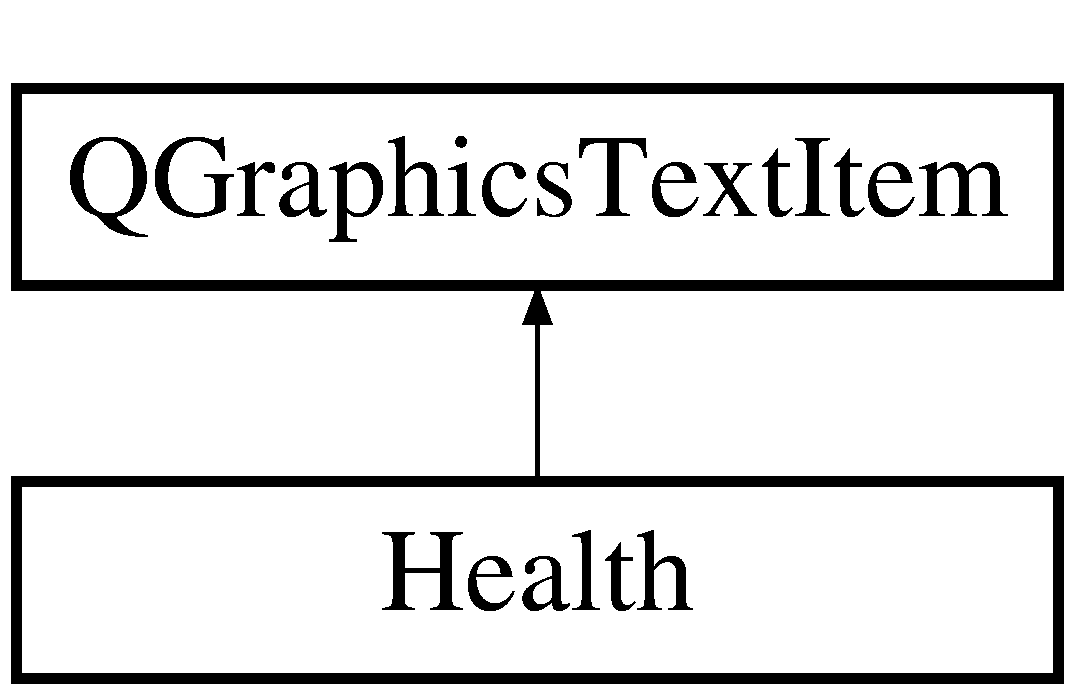
\includegraphics[height=2.000000cm]{class_health}
\end{center}
\end{figure}
\subsection*{Public Member Functions}
\begin{DoxyCompactItemize}
\item 
\hyperlink{class_health_af8daf3e4533a91b1987d2297dd765208}{Health} (Q\+Graphics\+Item $\ast$parent=0)
\begin{DoxyCompactList}\small\item\em Creates the health score. \end{DoxyCompactList}\item 
void \hyperlink{class_health_a15836492efb60f8c61151d35379768d2}{decrease} ()
\begin{DoxyCompactList}\small\item\em Decreases health when player collides with enemy. \end{DoxyCompactList}\item 
int \hyperlink{class_health_adc5f045b9f6937c592e196821d7a6878}{get\+Health} ()
\begin{DoxyCompactList}\small\item\em Returns the health score. \end{DoxyCompactList}\end{DoxyCompactItemize}
\subsection*{Private Attributes}
\begin{DoxyCompactItemize}
\item 
int \hyperlink{class_health_a24ea36e28b6def54066e6164f97544b6}{health}\hypertarget{class_health_a24ea36e28b6def54066e6164f97544b6}{}\label{class_health_a24ea36e28b6def54066e6164f97544b6}

\begin{DoxyCompactList}\small\item\em Contains the health score. \end{DoxyCompactList}\end{DoxyCompactItemize}


\subsection{Constructor \& Destructor Documentation}
\index{Health@{Health}!Health@{Health}}
\index{Health@{Health}!Health@{Health}}
\subsubsection[{\texorpdfstring{Health(\+Q\+Graphics\+Item $\ast$parent=0)}{Health(QGraphicsItem *parent=0)}}]{\setlength{\rightskip}{0pt plus 5cm}Health\+::\+Health (
\begin{DoxyParamCaption}
\item[{Q\+Graphics\+Item $\ast$}]{parent = {\ttfamily 0}}
\end{DoxyParamCaption}
)}\hypertarget{class_health_af8daf3e4533a91b1987d2297dd765208}{}\label{class_health_af8daf3e4533a91b1987d2297dd765208}


Creates the health score. 

initialize the health to 100

draw the text

$<$ \hyperlink{class_health}{Health}\+: 100 

\subsection{Member Function Documentation}
\index{Health@{Health}!decrease@{decrease}}
\index{decrease@{decrease}!Health@{Health}}
\subsubsection[{\texorpdfstring{decrease()}{decrease()}}]{\setlength{\rightskip}{0pt plus 5cm}void Health\+::decrease (
\begin{DoxyParamCaption}
{}
\end{DoxyParamCaption}
)}\hypertarget{class_health_a15836492efb60f8c61151d35379768d2}{}\label{class_health_a15836492efb60f8c61151d35379768d2}


Decreases health when player collides with enemy. 

Decreases the health. $<$ \hyperlink{class_health}{Health}\+: 99

$<$ Dead, display game over \index{Health@{Health}!get\+Health@{get\+Health}}
\index{get\+Health@{get\+Health}!Health@{Health}}
\subsubsection[{\texorpdfstring{get\+Health()}{getHealth()}}]{\setlength{\rightskip}{0pt plus 5cm}int Health\+::get\+Health (
\begin{DoxyParamCaption}
{}
\end{DoxyParamCaption}
)}\hypertarget{class_health_adc5f045b9f6937c592e196821d7a6878}{}\label{class_health_adc5f045b9f6937c592e196821d7a6878}


Returns the health score. 

Returns the health. 

The documentation for this class was generated from the following files\+:\begin{DoxyCompactItemize}
\item 
/\+Users/\+Katherine/\+Desktop/\+P\+I\+C 10\+C -\/ Winter 2015/\+Treasure Run Submission -\/ Hw8/health.\+h\item 
/\+Users/\+Katherine/\+Desktop/\+P\+I\+C 10\+C -\/ Winter 2015/\+Treasure Run Submission -\/ Hw8/health.\+cpp\end{DoxyCompactItemize}

\hypertarget{class_main_window}{}\section{Main\+Window Class Reference}
\label{class_main_window}\index{Main\+Window@{Main\+Window}}
Inheritance diagram for Main\+Window\+:\begin{figure}[H]
\begin{center}
\leavevmode
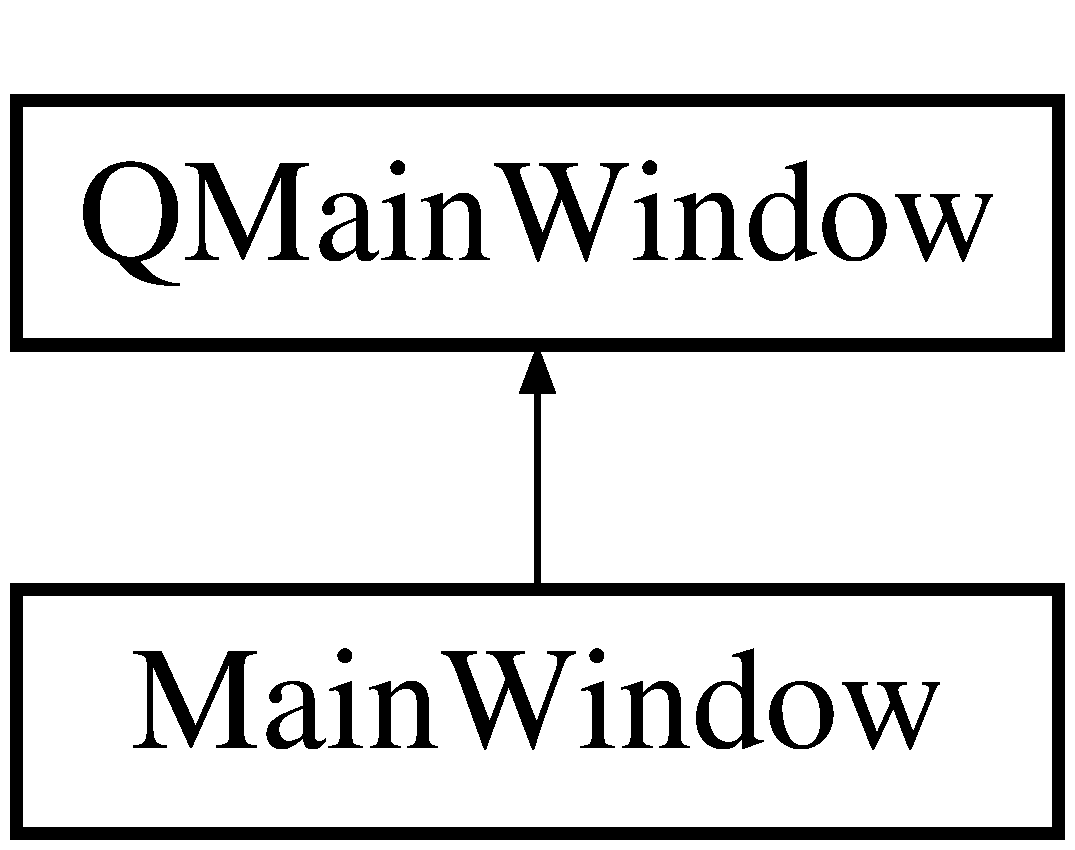
\includegraphics[height=2.000000cm]{class_main_window}
\end{center}
\end{figure}
\subsection*{Public Member Functions}
\begin{DoxyCompactItemize}
\item 
{\bfseries Main\+Window} (Q\+Widget $\ast$parent=0)\hypertarget{class_main_window_a8b244be8b7b7db1b08de2a2acb9409db}{}\label{class_main_window_a8b244be8b7b7db1b08de2a2acb9409db}

\end{DoxyCompactItemize}
\subsection*{Private Slots}
\begin{DoxyCompactItemize}
\item 
void \hyperlink{class_main_window_a4de79c63c7fa0b8d7c468ac71f20be81}{on\+\_\+push\+Button\+\_\+clicked} ()
\begin{DoxyCompactList}\small\item\em Pushbutton Begin that starts the game when clicked. \end{DoxyCompactList}\end{DoxyCompactItemize}
\subsection*{Private Attributes}
\begin{DoxyCompactItemize}
\item 
Ui\+::\+Main\+Window $\ast$ {\bfseries ui}\hypertarget{class_main_window_a35466a70ed47252a0191168126a352a5}{}\label{class_main_window_a35466a70ed47252a0191168126a352a5}

\end{DoxyCompactItemize}


\subsection{Member Function Documentation}
\index{Main\+Window@{Main\+Window}!on\+\_\+push\+Button\+\_\+clicked@{on\+\_\+push\+Button\+\_\+clicked}}
\index{on\+\_\+push\+Button\+\_\+clicked@{on\+\_\+push\+Button\+\_\+clicked}!Main\+Window@{Main\+Window}}
\subsubsection[{\texorpdfstring{on\+\_\+push\+Button\+\_\+clicked}{on_pushButton_clicked}}]{\setlength{\rightskip}{0pt plus 5cm}void Main\+Window\+::on\+\_\+push\+Button\+\_\+clicked (
\begin{DoxyParamCaption}
{}
\end{DoxyParamCaption}
)\hspace{0.3cm}{\ttfamily [private]}, {\ttfamily [slot]}}\hypertarget{class_main_window_a4de79c63c7fa0b8d7c468ac71f20be81}{}\label{class_main_window_a4de79c63c7fa0b8d7c468ac71f20be81}


Pushbutton Begin that starts the game when clicked. 

$<$ Opening the game 

The documentation for this class was generated from the following files\+:\begin{DoxyCompactItemize}
\item 
/\+Users/\+Katherine/\+Desktop/\+P\+I\+C 10\+C -\/ Winter 2015/\+Treasure Run Submission -\/ Hw8/mainwindow.\+h\item 
/\+Users/\+Katherine/\+Desktop/\+P\+I\+C 10\+C -\/ Winter 2015/\+Treasure Run Submission -\/ Hw8/mainwindow.\+cpp\end{DoxyCompactItemize}

\hypertarget{class_player}{}\section{Player Class Reference}
\label{class_player}\index{Player@{Player}}


{\ttfamily \#include $<$player.\+h$>$}

Inheritance diagram for Player\+:\begin{figure}[H]
\begin{center}
\leavevmode
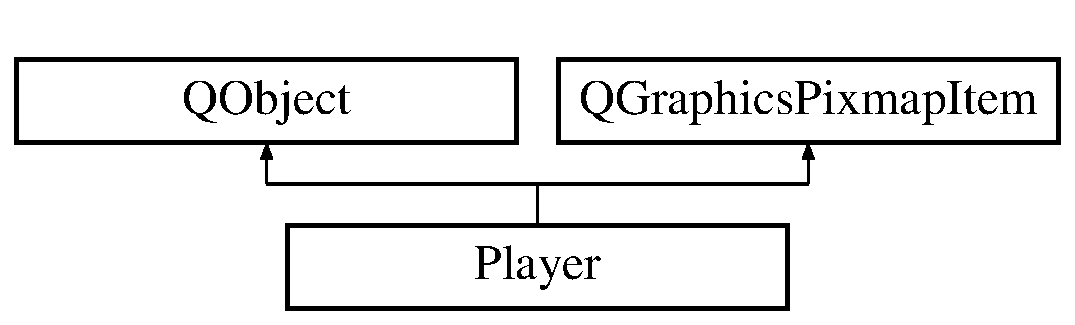
\includegraphics[height=2.000000cm]{class_player}
\end{center}
\end{figure}
\subsection*{Public Slots}
\begin{DoxyCompactItemize}
\item 
void \hyperlink{class_player_aeed92c166b9d0e272586baf3d23abe73}{spawn\+Enemies} ()
\begin{DoxyCompactList}\small\item\em Function that spawns enemies. \end{DoxyCompactList}\item 
void \hyperlink{class_player_a3380dce486a55b2dc5022416780495bb}{spawn\+Treasure} ()
\begin{DoxyCompactList}\small\item\em Function that spawns treasure. \end{DoxyCompactList}\end{DoxyCompactItemize}
\subsection*{Public Member Functions}
\begin{DoxyCompactItemize}
\item 
\hyperlink{class_player_a4d193d415c83e385e41f5daf4cc5b06c}{Player} (Q\+Graphics\+Item $\ast$parent=0)
\begin{DoxyCompactList}\small\item\em $<$ for public slots \end{DoxyCompactList}\item 
void \hyperlink{class_player_a4d269c4118c29b0ee85c1e0f674260ee}{key\+Press\+Event} (Q\+Key\+Event $\ast$event)
\begin{DoxyCompactList}\small\item\em When a specific key is pressed, the player will move. \end{DoxyCompactList}\end{DoxyCompactItemize}


\subsection{Detailed Description}
Name Katherine Wang Final \hyperlink{class_game}{Game} Assignment Description\+: This class creates the player (the character) and also allows the player to control his character through the arrow keys. Also spawns enemies. 

\subsection{Constructor \& Destructor Documentation}
\index{Player@{Player}!Player@{Player}}
\index{Player@{Player}!Player@{Player}}
\subsubsection[{\texorpdfstring{Player(\+Q\+Graphics\+Item $\ast$parent=0)}{Player(QGraphicsItem *parent=0)}}]{\setlength{\rightskip}{0pt plus 5cm}Player\+::\+Player (
\begin{DoxyParamCaption}
\item[{Q\+Graphics\+Item $\ast$}]{parent = {\ttfamily 0}}
\end{DoxyParamCaption}
)}\hypertarget{class_player_a4d193d415c83e385e41f5daf4cc5b06c}{}\label{class_player_a4d193d415c83e385e41f5daf4cc5b06c}


$<$ for public slots 

Name Katherine Wang Assignment 5 Description\+: This class creates the player (the character). Also allows movement of the character and spawns enemies. set the player image 

\subsection{Member Function Documentation}
\index{Player@{Player}!key\+Press\+Event@{key\+Press\+Event}}
\index{key\+Press\+Event@{key\+Press\+Event}!Player@{Player}}
\subsubsection[{\texorpdfstring{key\+Press\+Event(\+Q\+Key\+Event $\ast$event)}{keyPressEvent(QKeyEvent *event)}}]{\setlength{\rightskip}{0pt plus 5cm}void Player\+::key\+Press\+Event (
\begin{DoxyParamCaption}
\item[{Q\+Key\+Event $\ast$}]{event}
\end{DoxyParamCaption}
)}\hypertarget{class_player_a4d269c4118c29b0ee85c1e0f674260ee}{}\label{class_player_a4d269c4118c29b0ee85c1e0f674260ee}


When a specific key is pressed, the player will move. 

---Moving the player to the Left---//

If the position of the player is greater than 0 on the x-\/axis, to avoid going off screen

move the character to the left by 10 pixels

---Moving the player right---//

If the position of the player is less than 800 on the y-\/axis, to avoid going off screen

move the character to the right by 10 pixels \index{Player@{Player}!spawn\+Enemies@{spawn\+Enemies}}
\index{spawn\+Enemies@{spawn\+Enemies}!Player@{Player}}
\subsubsection[{\texorpdfstring{spawn\+Enemies}{spawnEnemies}}]{\setlength{\rightskip}{0pt plus 5cm}void Player\+::spawn\+Enemies (
\begin{DoxyParamCaption}
{}
\end{DoxyParamCaption}
)\hspace{0.3cm}{\ttfamily [slot]}}\hypertarget{class_player_aeed92c166b9d0e272586baf3d23abe73}{}\label{class_player_aeed92c166b9d0e272586baf3d23abe73}


Function that spawns enemies. 

Creates an enemy. \index{Player@{Player}!spawn\+Treasure@{spawn\+Treasure}}
\index{spawn\+Treasure@{spawn\+Treasure}!Player@{Player}}
\subsubsection[{\texorpdfstring{spawn\+Treasure}{spawnTreasure}}]{\setlength{\rightskip}{0pt plus 5cm}void Player\+::spawn\+Treasure (
\begin{DoxyParamCaption}
{}
\end{DoxyParamCaption}
)\hspace{0.3cm}{\ttfamily [slot]}}\hypertarget{class_player_a3380dce486a55b2dc5022416780495bb}{}\label{class_player_a3380dce486a55b2dc5022416780495bb}


Function that spawns treasure. 

Creates a treasure chest. 

The documentation for this class was generated from the following files\+:\begin{DoxyCompactItemize}
\item 
/\+Users/\+Katherine/\+Desktop/\+P\+I\+C 10\+C -\/ Winter 2015/\+Treasure Run Submission -\/ Hw8/player.\+h\item 
/\+Users/\+Katherine/\+Desktop/\+P\+I\+C 10\+C -\/ Winter 2015/\+Treasure Run Submission -\/ Hw8/player.\+cpp\end{DoxyCompactItemize}

\hypertarget{class_score}{}\section{Score Class Reference}
\label{class_score}\index{Score@{Score}}
Inheritance diagram for Score\+:\begin{figure}[H]
\begin{center}
\leavevmode
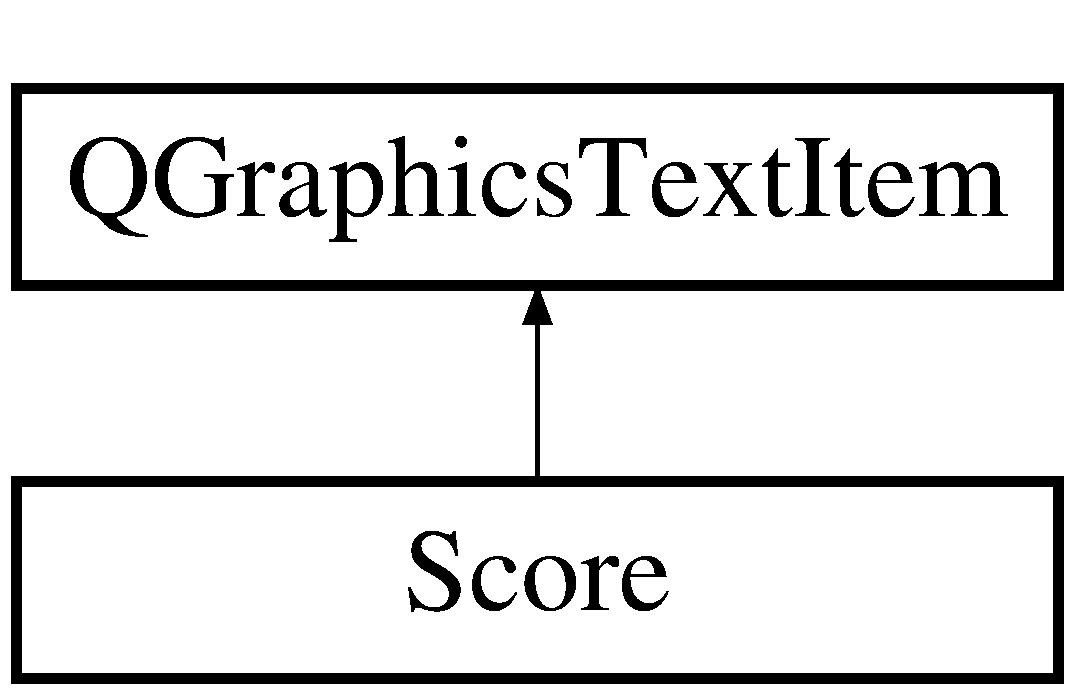
\includegraphics[height=2.000000cm]{class_score}
\end{center}
\end{figure}
\subsection*{Public Member Functions}
\begin{DoxyCompactItemize}
\item 
\hyperlink{class_score_af7c3392a27388a66b8a94448a995634d}{Score} (Q\+Graphics\+Item $\ast$parent=0)
\item 
void \hyperlink{class_score_ab5dbfab6935903c075509546878cfbda}{increase} ()
\begin{DoxyCompactList}\small\item\em Increases score when player collides with treasure chest. \end{DoxyCompactList}\item 
int \hyperlink{class_score_a8627c93270c188a3fd28a25b1d07a9e7}{get\+Score} ()
\begin{DoxyCompactList}\small\item\em Returns the total score. \end{DoxyCompactList}\end{DoxyCompactItemize}
\subsection*{Private Attributes}
\begin{DoxyCompactItemize}
\item 
int \hyperlink{class_score_a331b0927105c83ba760954eff6cf9fe9}{score}\hypertarget{class_score_a331b0927105c83ba760954eff6cf9fe9}{}\label{class_score_a331b0927105c83ba760954eff6cf9fe9}

\begin{DoxyCompactList}\small\item\em Contains the score. \end{DoxyCompactList}\end{DoxyCompactItemize}


\subsection{Constructor \& Destructor Documentation}
\index{Score@{Score}!Score@{Score}}
\index{Score@{Score}!Score@{Score}}
\subsubsection[{\texorpdfstring{Score(\+Q\+Graphics\+Item $\ast$parent=0)}{Score(QGraphicsItem *parent=0)}}]{\setlength{\rightskip}{0pt plus 5cm}Score\+::\+Score (
\begin{DoxyParamCaption}
\item[{Q\+Graphics\+Item $\ast$}]{parent = {\ttfamily 0}}
\end{DoxyParamCaption}
)}\hypertarget{class_score_af7c3392a27388a66b8a94448a995634d}{}\label{class_score_af7c3392a27388a66b8a94448a995634d}
initialize the score to 0

draw the text 

\subsection{Member Function Documentation}
\index{Score@{Score}!get\+Score@{get\+Score}}
\index{get\+Score@{get\+Score}!Score@{Score}}
\subsubsection[{\texorpdfstring{get\+Score()}{getScore()}}]{\setlength{\rightskip}{0pt plus 5cm}int Score\+::get\+Score (
\begin{DoxyParamCaption}
{}
\end{DoxyParamCaption}
)}\hypertarget{class_score_a8627c93270c188a3fd28a25b1d07a9e7}{}\label{class_score_a8627c93270c188a3fd28a25b1d07a9e7}


Returns the total score. 

Returns score publically. \index{Score@{Score}!increase@{increase}}
\index{increase@{increase}!Score@{Score}}
\subsubsection[{\texorpdfstring{increase()}{increase()}}]{\setlength{\rightskip}{0pt plus 5cm}void Score\+::increase (
\begin{DoxyParamCaption}
{}
\end{DoxyParamCaption}
)}\hypertarget{class_score_ab5dbfab6935903c075509546878cfbda}{}\label{class_score_ab5dbfab6935903c075509546878cfbda}


Increases score when player collides with treasure chest. 

Increases the score when the player collides with a treasure chest. $<$ increasing score

If the player wins, display the win prompt 

The documentation for this class was generated from the following files\+:\begin{DoxyCompactItemize}
\item 
/\+Users/\+Katherine/\+Desktop/\+P\+I\+C 10\+C -\/ Winter 2015/\+Treasure Run Submission -\/ Hw8/score.\+h\item 
/\+Users/\+Katherine/\+Desktop/\+P\+I\+C 10\+C -\/ Winter 2015/\+Treasure Run Submission -\/ Hw8/score.\+cpp\end{DoxyCompactItemize}

\hypertarget{class_weapon}{}\section{Weapon Class Reference}
\label{class_weapon}\index{Weapon@{Weapon}}


$<$For implementing graphics  




{\ttfamily \#include $<$weapon.\+h$>$}

Inheritance diagram for Weapon\+:\begin{figure}[H]
\begin{center}
\leavevmode
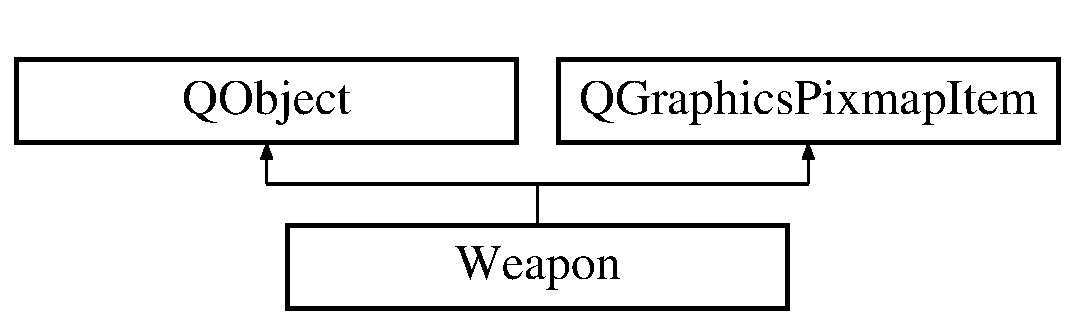
\includegraphics[height=2.000000cm]{class_weapon}
\end{center}
\end{figure}
\subsection*{Public Slots}
\begin{DoxyCompactItemize}
\item 
void \hyperlink{class_weapon_a1d62683b1b6dc0795420c7da6f141437}{move} ()
\begin{DoxyCompactList}\small\item\em Moves the treasure chest down. \end{DoxyCompactList}\end{DoxyCompactItemize}
\subsection*{Public Member Functions}
\begin{DoxyCompactItemize}
\item 
\hyperlink{class_weapon_a42dbc46dd70319a24763992c4ebbd396}{Weapon} ()
\begin{DoxyCompactList}\small\item\em Spawns a tresure chest that will randomly generate a new weapon damage. \end{DoxyCompactList}\end{DoxyCompactItemize}


\subsection{Detailed Description}
$<$For implementing graphics 

The weapon file implements treasure chests into the game, which are required to win the game.$<$for signalling slots 

\subsection{Constructor \& Destructor Documentation}
\index{Weapon@{Weapon}!Weapon@{Weapon}}
\index{Weapon@{Weapon}!Weapon@{Weapon}}
\subsubsection[{\texorpdfstring{Weapon()}{Weapon()}}]{\setlength{\rightskip}{0pt plus 5cm}Weapon\+::\+Weapon (
\begin{DoxyParamCaption}
{}
\end{DoxyParamCaption}
)}\hypertarget{class_weapon_a42dbc46dd70319a24763992c4ebbd396}{}\label{class_weapon_a42dbc46dd70319a24763992c4ebbd396}


Spawns a tresure chest that will randomly generate a new weapon damage. 

$<$ Set a random position for the treasure chest

$<$ Draw the rectangle of the treasure chest

Connecting the treasure chest

$<$ object whose signal you want to connect, constructor, move.

$<$ setting timer\textquotesingle{}s time to 50 milliseconds. 

\subsection{Member Function Documentation}
\index{Weapon@{Weapon}!move@{move}}
\index{move@{move}!Weapon@{Weapon}}
\subsubsection[{\texorpdfstring{move}{move}}]{\setlength{\rightskip}{0pt plus 5cm}void Weapon\+::move (
\begin{DoxyParamCaption}
{}
\end{DoxyParamCaption}
)\hspace{0.3cm}{\ttfamily [slot]}}\hypertarget{class_weapon_a1d62683b1b6dc0795420c7da6f141437}{}\label{class_weapon_a1d62683b1b6dc0795420c7da6f141437}


Moves the treasure chest down. 

if treasure\+Chest collides with player, destroy the chest and give the player a random weapon

playing the treasure chest collection sound

If treasure chest collides with player, remove the chest

moving chest down

$<$ x() = current x, y() = current y

delete the enemy when it\textquotesingle{}s off the screen 

The documentation for this class was generated from the following files\+:\begin{DoxyCompactItemize}
\item 
/\+Users/\+Katherine/\+Desktop/\+P\+I\+C 10\+C -\/ Winter 2015/\+Treasure Run Submission -\/ Hw8/weapon.\+h\item 
/\+Users/\+Katherine/\+Desktop/\+P\+I\+C 10\+C -\/ Winter 2015/\+Treasure Run Submission -\/ Hw8/weapon.\+cpp\end{DoxyCompactItemize}

\hypertarget{class_weaponscore}{}\section{Weaponscore Class Reference}
\label{class_weaponscore}\index{Weaponscore@{Weaponscore}}
Inheritance diagram for Weaponscore\+:\begin{figure}[H]
\begin{center}
\leavevmode
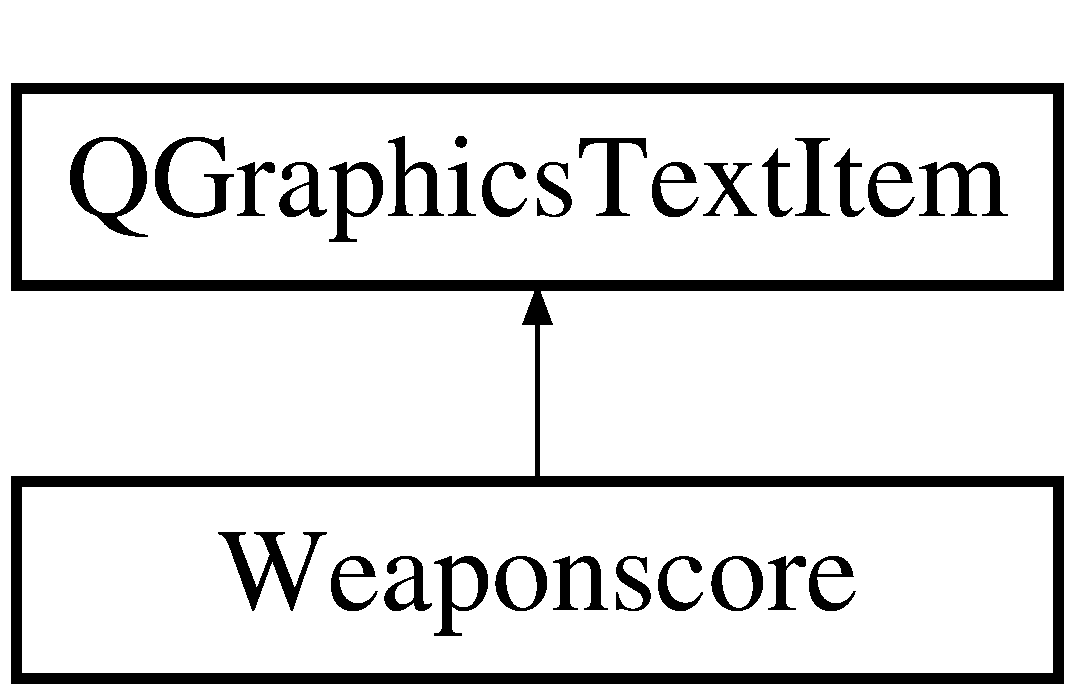
\includegraphics[height=2.000000cm]{class_weaponscore}
\end{center}
\end{figure}
\subsection*{Public Member Functions}
\begin{DoxyCompactItemize}
\item 
{\bfseries Weaponscore} (Q\+Graphics\+Item $\ast$parent=0)\hypertarget{class_weaponscore_afac1c5e0243854098e09ffa5139f4e5b}{}\label{class_weaponscore_afac1c5e0243854098e09ffa5139f4e5b}

\item 
void {\bfseries increase} ()\hypertarget{class_weaponscore_a555c98168d06757088feadbb3d978d77}{}\label{class_weaponscore_a555c98168d06757088feadbb3d978d77}

\item 
int {\bfseries get\+Damage} ()\hypertarget{class_weaponscore_a9dc99bef95de474087f9e08eb178a4bd}{}\label{class_weaponscore_a9dc99bef95de474087f9e08eb178a4bd}

\end{DoxyCompactItemize}
\subsection*{Private Attributes}
\begin{DoxyCompactItemize}
\item 
int {\bfseries damage\+\_\+score}\hypertarget{class_weaponscore_aaf17b1bc5499cf076e19d70efcd91cd4}{}\label{class_weaponscore_aaf17b1bc5499cf076e19d70efcd91cd4}

\end{DoxyCompactItemize}
\subsection*{Friends}
\begin{DoxyCompactItemize}
\item 
class {\bfseries Weapon}\hypertarget{class_weaponscore_ab356dbee0f1e915287732c65e8ef61e1}{}\label{class_weaponscore_ab356dbee0f1e915287732c65e8ef61e1}

\end{DoxyCompactItemize}


The documentation for this class was generated from the following files\+:\begin{DoxyCompactItemize}
\item 
/\+Users/\+Katherine/\+Desktop/\+P\+I\+C 10\+C -\/ Winter 2015/\+Treasure Run Submission -\/ Hw8/weaponscore.\+h\item 
/\+Users/\+Katherine/\+Desktop/\+P\+I\+C 10\+C -\/ Winter 2015/\+Treasure Run Submission -\/ Hw8/weaponscore.\+cpp\end{DoxyCompactItemize}

%--- End generated contents ---

% Index
\backmatter
\newpage
\phantomsection
\clearemptydoublepage
\addcontentsline{toc}{chapter}{Index}
\printindex

\end{document}
